\chapter{Communication Protocol}

\section{FreeRTOS}

Ideally FreeRTOS tasks should operate with as much isolation as possible, with each task performing a specific function with different priority levels. In the case of a communication protocol, the overall task is inherently sequential so this leads to FreeRTOS being used in a sequential way with all tasks operating at real-time priority level. 

FreeRTOS was chosen because of the following benefits:

\begin{enumerate}
\item Segmentation of code into specific tasks provides readable code for future users.
\item FreeRTOS task configuration provides a framework for future embedded robotic control systems as well as easily reconfigurable code.
\item Semaphores and queues lend themselves to sequential reception and processing of packets at predefined intervals very well.
\item Isolation of tasks provides easy debugging of communication issues.
\end{enumerate}

\subsection{Heartbeat Task}
\subsection{PC TX Task}
\subsection{PC RX Task}
\subsection{TX Motor Task}
\subsection{RX Motor Task}
\subsection{Controller Task}

\subsection{FreeRTOS Timing}

The default 1000 Hz tick rate was overridden with a tick rate of 5000 Hz to enable more fine tuned packet timing and delays. The timing configuration can be seen in \cref{listing:FreeRTOS timing}. 

In order to achieve a control loop rate of 200 Hz, a sampling time of 5 ms or 25 ticks was used.

\section{Packet Encoding and Decoding}

SeqBits bits 2-5 switch case

\begin{figure}
\centering
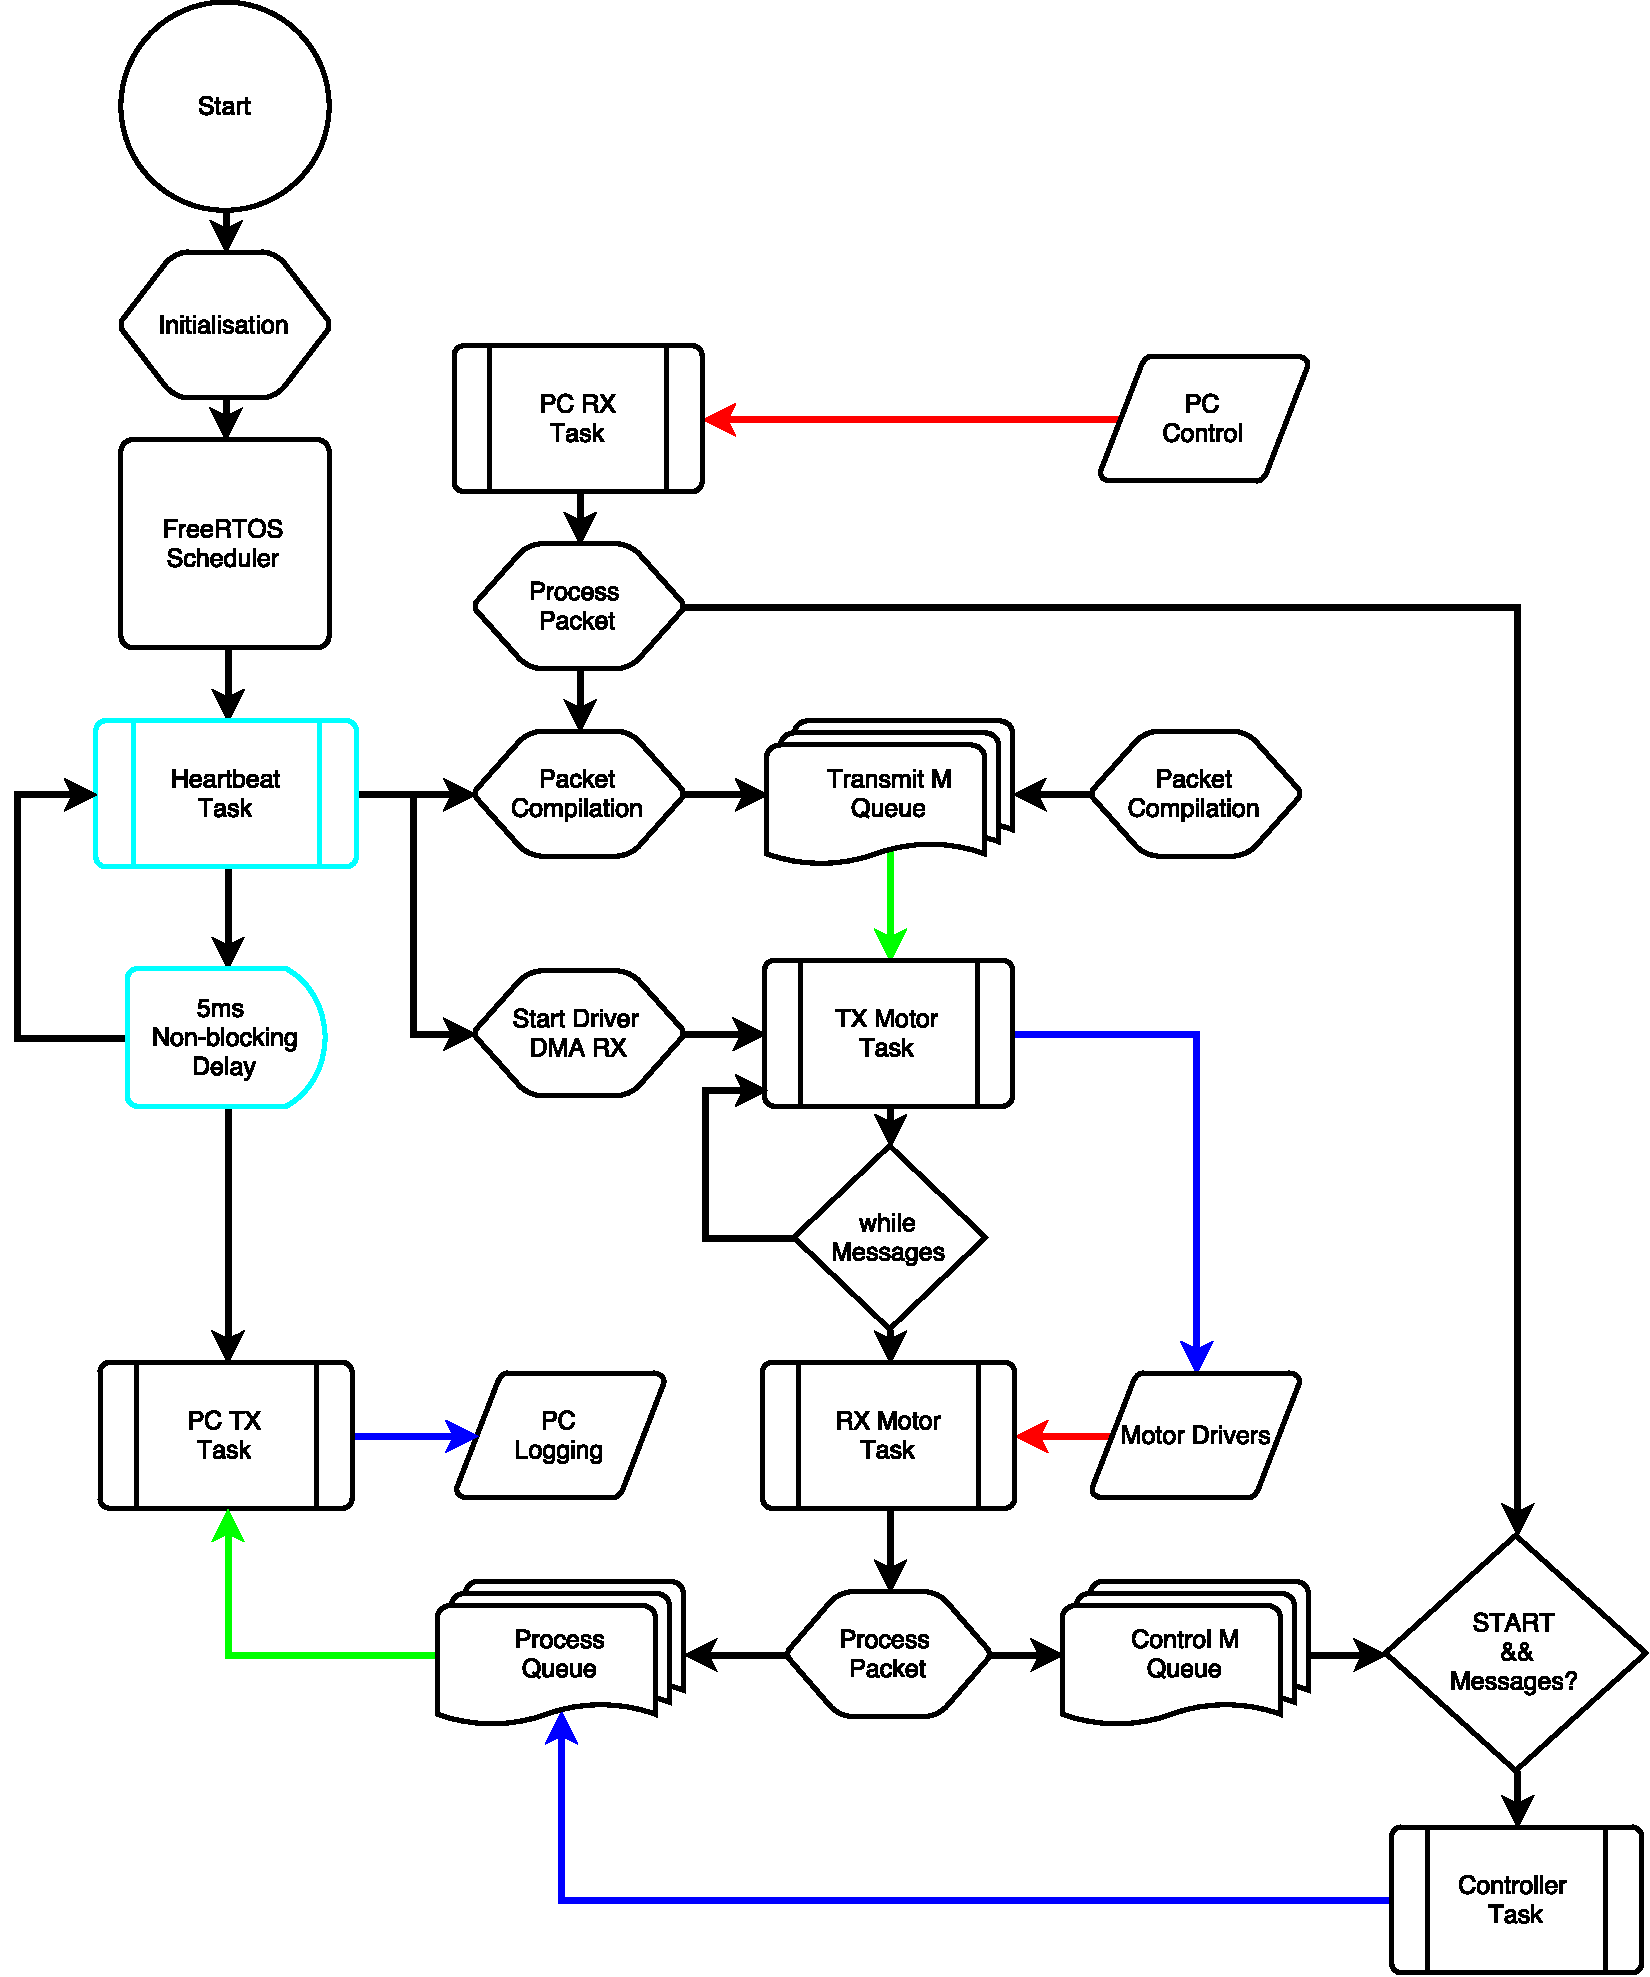
\includegraphics[width=1\textwidth]{images/comms/communication-flow-diagram.pdf} 
\caption{FreeRTOS communication protocol flow diagram.}
\label{fig:FreeRTOS communication protocol flow diagram.}
\end{figure}

\begin{figure}
\centering
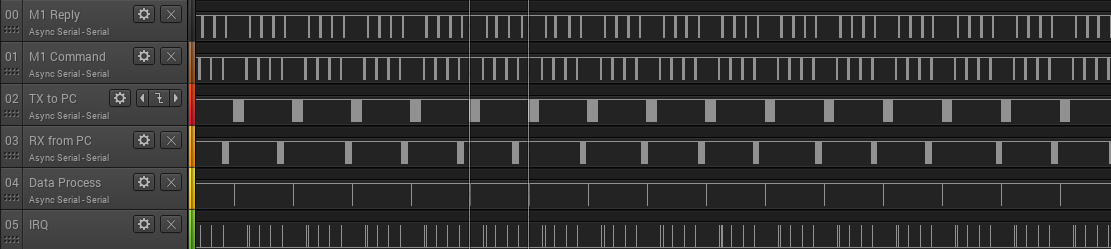
\includegraphics[width=1\textwidth]{images/comms/pc-packet-timing-data} 
\caption{Communication protocol packet timing with 5 ms sampling rate.}
\label{fig:packet-timing.}
\end{figure}

\begin{table}
\centering
\begin{tabular}{llllll}
\textbf{Command}       & \textbf{Index} & \textbf{Op-Code} & \textbf{TX CB} & \textbf{TX CRC1} & \textbf{RX  CB} \\
\textbf{Kill Bridge}   & 1              & 0001             & 0x06           & 0xCBB6           & 0x04            \\
\textbf{Write Enable}  & 2              & 0010             & 0x0A           & 0x3624           & 0x08            \\
\textbf{Bridge Enable} & 3              & 0100             & 0x12           & 0x1AE0           & 0x10            \\
\textbf{Set Current}   & 4              & 0011             & 0x0E           & 0xBF7B           & 0x0C            \\
\textbf{Read Current}  & 5              & 1100             & 0x31           & 0x9772           & 0x32            \\
\textbf{Read Position} & 6              & 1111             & 0x3D           & 0xD310           & 0x3E            \\
\textbf{Read Velocity} & 7              & 0101             & 0x15           & 0x5EAF           & 0x16            \\
\textbf{Set Position}  & 8              & 1010             & 0x2A           & 0x42C4           & 0x28           
\end{tabular}
\caption{Motor driver command protocol.}
\label{tab:motor-driver-protocol}
\end{table}